% see https://tex.stackexchange.com/a/208409/145331
\begin{frame}[fragile]{\SAPFEC{} problem}

    \only<1>{
        \begin{center}
            \textbf{Original Map}

            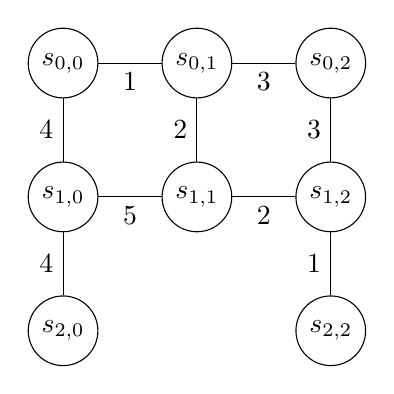
\begin{tikzpicture}
                \tikzset{Vertex/.style={%
                    shape=circle,%
                    draw=black,%
                    minimum size=10pt,%
                    radius=1cm,%
                    inner sep=3pt,%
                    node distance=1.7cm,%
                }}
        
                \node[Vertex] (v00) at (0,0) {$s_{0,0}$};
                \node[Vertex, right of=v00] (v01) {$s_{0,1}$};
                \node[Vertex, right of=v01] (v02) {$s_{0,2}$};
                \node[Vertex, below of=v00] (v10) {$s_{1,0}$};
                \node[Vertex, right of=v10] (v11) {$s_{1,1}$};
                \node[Vertex, right of=v11] (v12) {$s_{1,2}$};
                \node[Vertex, below of=v10] (v20) {$s_{2,0}$};
                \node[Vertex, below of=v12] (v22) {$s_{2,2}$};
        
                \path (v00) edge[-.] node[below]{1} (v01);
                \path (v01) edge[-.] node[below]{3} (v02);
                \path (v10) edge[-.] node[below]{5} (v11);
                \path (v11) edge[-.] node[below]{2} (v12);
                \path (v00) edge[-.] node[left]{4} (v10);
                \path (v10) edge[-.] node[left]{4} (v20);
                \path (v01) edge[-.] node[left]{2} (v11);
                \path (v02) edge[-.] node[left]{3} (v12);
                \path (v12) edge[-.] node[left]{1} (v22);
            \end{tikzpicture}
        \end{center}
    }%
    \only<2>{
        \begin{center}
            \textbf{Original Map}

            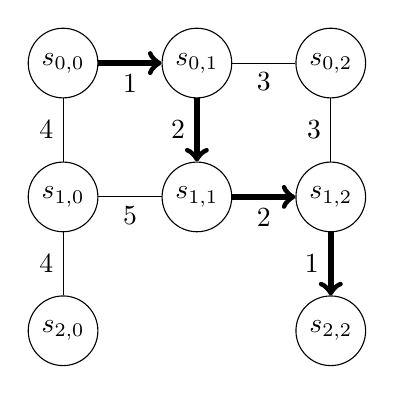
\begin{tikzpicture}
                \tikzset{Vertex/.style={%
                    shape=circle,%
                    draw=black,%
                    minimum size=10pt,%
                    radius=1cm,%
                    inner sep=3pt,%
                    node distance=1.7cm,%
                }}
        
                \node[Vertex] (v00) at (0,0) {$s_{0,0}$};
                \node[Vertex, right of=v00] (v01) {$s_{0,1}$};
                \node[Vertex, right of=v01] (v02) {$s_{0,2}$};
                \node[Vertex, below of=v00] (v10) {$s_{1,0}$};
                \node[Vertex, right of=v10] (v11) {$s_{1,1}$};
                \node[Vertex, right of=v11] (v12) {$s_{1,2}$};
                \node[Vertex, below of=v10] (v20) {$s_{2,0}$};
                \node[Vertex, below of=v12] (v22) {$s_{2,2}$};
        
                \path (v00) edge[->,line width=2pt] node[below]{1} (v01);
                \path (v01) edge[-.] node[below]{3} (v02);
                \path (v10) edge[-.] node[below]{5} (v11);
                \path (v11) edge[->,line width=2pt] node[below]{2} (v12);
                \path (v00) edge[-.] node[left]{4} (v10);
                \path (v10) edge[-.] node[left]{4} (v20);
                \path (v01) edge[->,line width=2pt] node[left]{2} (v11);
                \path (v02) edge[-.] node[left]{3} (v12);
                \path (v12) edge[->,line width=2pt] node[left]{1} (v22);
            \end{tikzpicture}

            $$s_{0,0} \rightarrow s_{0,1} \rightarrow s_{1,1} \rightarrow s_{1,2} \rightarrow s_{2,2}$$
        \end{center}
    }%
    \only<3>{
        \begin{center}
            \textbf{Perturbated Map}

            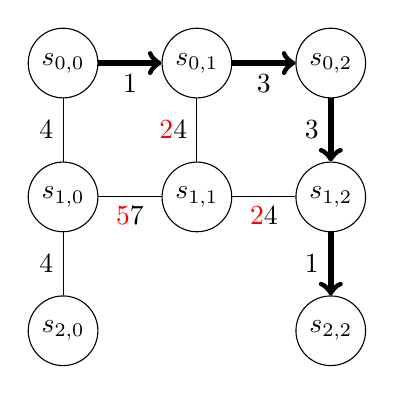
\begin{tikzpicture}
                \tikzset{Vertex/.style={%
                    shape=circle,%
                    draw=black,%
                    minimum size=10pt,%
                    radius=1cm,%
                    inner sep=3pt,%
                    node distance=1.7cm,%
                }}
        
                \node[Vertex] (v00) at (0,0) {$s_{0,0}$};
                \node[Vertex, right of=v00] (v01) {$s_{0,1}$};
                \node[Vertex, right of=v01] (v02) {$s_{0,2}$};
                \node[Vertex, below of=v00] (v10) {$s_{1,0}$};
                \node[Vertex, right of=v10] (v11) {$s_{1,1}$};
                \node[Vertex, right of=v11] (v12) {$s_{1,2}$};
                \node[Vertex, below of=v10] (v20) {$s_{2,0}$};
                \node[Vertex, below of=v12] (v22) {$s_{2,2}$};
        
                \path (v00) edge[->,line width=2pt] node[below]{1} (v01);
                \path (v01) edge[->,line width=2pt] node[below]{3} (v02);
                \path (v10) edge[-.] node[below]{{\color{red} \xcancel{5}}{7}} (v11);
                \path (v11) edge[-.] node[below]{{\color{red} \xcancel{2}}{4}} (v12);
                \path (v00) edge[-.] node[left]{4} (v10);
                \path (v10) edge[-.] node[left]{4} (v20);
                \path (v01) edge[-.] node[left]{{\color{red} \xcancel{2}}{4}} (v11);
                \path (v02) edge[->,line width=2pt] node[left]{3} (v12);
                \path (v12) edge[->,line width=2pt] node[left]{1} (v22);
            \end{tikzpicture}

            $$s_{0,0} \rightarrow s_{0,1} \rightarrow s_{0,2} \rightarrow s_{1,2} \rightarrow s_{2,2}$$
        \end{center}
    }
    
\end{frame}

\begin{frame}{\SAPFEC{} context}
    \begin{itemize}
        \item Path planning episodes are independent;
        \item each episode has fixed start and target locations;
        \item graph map is known a priori.
    \end{itemize}
    
    \medskip
    Map edge costs changes (\textit{perturbations}):
    \begin{itemize}
        \item[-] Distribution over map unknown a priori;
        \item[-] \textbf{only increase} original edge costs (\eg{} routing in road networks, videogames);
        \item[-] detected at the beginning of each path planning episode and then assumed fixed.
    \end{itemize}
\end{frame}


\begin{frame}{\CPDSearch{} [Bono, Gerevini, Harabor, Stuckey, 2019]}
    \vspace{-8pt}
    \begin{block}{\CPDSearch{}}
        \A{} variant yielding bounded suboptimal solutions where \CPDPathsName{} are exploited for searching the perturbated map (for brevity, here we focus on the optimal working mode)
    \end{block}

    $s$, $t$ : start and target of path finding instance;
    
    $n$: a search node expanded during \CPDSearch{};

    \begin{coloredBlock}{Property}[OliveGreen][white]
        Each node $n$ has implicitly associated, via the CPD, a path to the given target $t$ which is optimal over the original graph (the \CPDPath{$n$}{$t$}).
    \end{coloredBlock}

    \vspace{-3pt}
    \begin{block}{}
        \begin{itemize}
            \item[-] $\CPDPathCostOriginal{n}{t}$: cost of \CPDPathName{} from $n$ to $t$ using the \textbf{original} weights;
            \item[-] $\CPDPathCostNew{n}{t}$: cost of \CPDPathName{} from $n$ to $t$ using the \textbf{perturbated} weights.
        \end{itemize} 
    \end{block}
    
\end{frame}

\begin{frame}{\CPDPathsName{} for deriving an admissible heuristic}

    \begin{itemize}
        \item Admissible heuristic: $\CPDPathCostOriginal{n}{t}$ is a lowerbound of the cost of an optimal path in the perturbated graph (perturbations increase costs).
        \begin{figure}
            \centering
            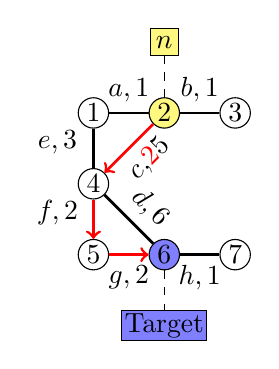
\begin{tikzpicture}
                \tikzset{Vertex/.style={%
                    shape=circle,%
                    draw=black,%
                    minimum size=10pt,%
                    radius=0.7cm,%
                    inner sep=1pt,%
                    node distance=0.9cm,%
                }}
                \tikzset{Note/.style={%
                    shape=rectangle,%
                    draw=black,%
                    minimum size=10pt,%
                    inner sep=1pt,%
                    node distance=0.9cm,%
                }}
            
                \node[Vertex] (1) {$1$};
                \node[Vertex, right of=1, fill=yellow!50] (2) {$2$};
                \node[Vertex, right of=2] (3) {$3$};
                \node[Vertex, below of=1] (4) {$4$};
                \node[Vertex, below of=4] (5) {$5$};
                \node[Vertex, right of=5, fill=blue!50] (6) {$6$};
                \node[Vertex, right of=6] (7) {$7$};

                \node[Note, above of=2, fill=yellow!50] (n) {$n$};
                \node[Note, below of=6, fill=blue!50] (target) {Target};

                \path (2) edge[-., dashed] (n);
                \path (6) edge[-., dashed] (target);
        
                \path (2) edge[-,line width=1pt] node[above]{\color{black}$a,1$} (1);
                \path (2) edge[-,line width=1pt] node[above]{\color{black}$b,1$} (3);
                \path (2) edge[->,line width=1pt, color=red] node[below,sloped,pos=0.4]{{\color{black} $c,$}{\color{red} \xcancel{2}}{\color{black}5}} (4);
                \path (4) edge[-,line width=1pt] node[above,sloped,pos=0.6]{\color{black}$d,6$} (6);
                \path (1) edge[-,line width=1pt] node[above,xshift=-13pt,yshift=-6pt]{\color{black}$e,3$} (4);
                \path (4) edge[->,line width=1pt, color=red] node[above,xshift=-13pt, yshift=-6pt]{\color{black}$f,2$} (5);
                \path (5) edge[->,line width=1pt, color=red] node[below]{\color{black}$g,2$} (6);
                \path (6) edge[-,line width=1pt] node[below]{\color{black}$h,1$} (7);
            \end{tikzpicture}
        \end{figure}
    \end{itemize}

\end{frame}

\begin{frame}{\CPDPathsName{} for early terminating the search}

    \textbf{Early search termination}: if the \CPDPath{$n$}{$t$} is not perturbated, then we already know an optimal path for going from $n$ to $t$ in the perturbated graph as well!
    \begin{minipage}{0.65\textwidth}

        \begin{center}
            if $\CPDPathCostNew{n}{t} = \CPDPathCostOriginal{n}{t}$
            
            $\downarrow$
            
            optimal solution is $\pathOnGraph{s}{n} \doublePlus{} \CPDPath{n}{t}$;

            \medskip

            $(s, t) = (2, 6)$
        
            $\CPDPathCostOriginal{4}{6} = 4$

            $\CPDPathCostNew{4}{6} = 4$
        \end{center}
    \end{minipage}\hfill%
    \begin{minipage}{0.35\textwidth}
        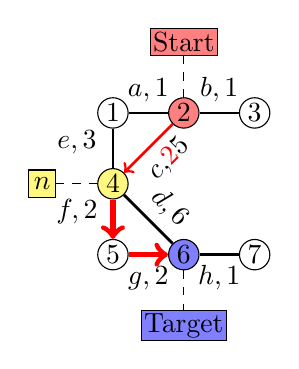
\begin{tikzpicture}
            \tikzset{Vertex/.style={%
                shape=circle,%
                draw=black,%
                minimum size=10pt,%
                radius=0.7cm,%
                inner sep=1pt,%
                node distance=0.9cm,%
            }}
            \tikzset{Note/.style={%
                shape=rectangle,%
                draw=black,%
                minimum size=10pt,%
                inner sep=1pt,%
                node distance=0.9cm,%
            }}
        
            \node[Vertex] (1) {$1$};
            \node[Vertex, right of=1, fill=red!50] (2) {$2$};
            \node[Vertex, right of=2] (3) {$3$};
            \node[Vertex, below of=1, fill=yellow!50] (4) {$4$};
            \node[Vertex, below of=4] (5) {$5$};
            \node[Vertex, right of=5, fill=blue!50] (6) {$6$};
            \node[Vertex, right of=6] (7) {$7$};

            \node[Note, above of=2, fill=red!50] (start) {Start};
            \node[Note, left of=4, fill=yellow!50] (n) {$n$};
            \node[Note, below of=6, fill=blue!50] (target) {Target};

            \path (2) edge[-., dashed] (start);
            \path (4) edge[-., dashed] (n);
            \path (6) edge[-., dashed] (target);
    
            \path (2) edge[-,line width=1pt] node[above]{\color{black}$a,1$} (1);
            \path (2) edge[-,line width=1pt] node[above]{\color{black}$b,1$} (3);
            \path (2) edge[->,line width=1pt, color=red] node[below,sloped,pos=0.4]{{\color{black} $c,$}{\color{red} \xcancel{2}}{\color{black}5}} (4);
            \path (4) edge[-,line width=1pt] node[above,sloped,pos=0.6]{\color{black}$d,6$} (6);
            \path (1) edge[-,line width=1pt] node[above,xshift=-13pt,yshift=-6pt]{\color{black}$e,3$} (4);
            \path (4) edge[->,line width=2pt, color=red] node[above,xshift=-13pt, yshift=-6pt]{\color{black}$f,2$} (5);
            \path (5) edge[->,line width=2pt, color=red] node[below]{\color{black}$g,2$} (6);
            \path (6) edge[-,line width=1pt] node[below]{\color{black}$h,1$} (7);
        \end{tikzpicture}
    \end{minipage}
\end{frame}

\begin{frame}{\CPDSearch{}}

    \begin{block}{\CPDSearch{}}
        \A{} variant yielding bounded suboptimal solutions where \CPDPathsName{} are exploited for searching the perturbated map (for brevity, we focus on the optimal working mode)
    \end{block}

    \begin{itemize}
        \item \CPDSearch{} maintains the best solution found and solution bounds (allows usage in anytime search);
        \item bounds computed thanks to $\CPDPathCostOriginal{n}{t}$ and $\CPDPathCostNew{n}{t}$;
        \item a threshold can be set to make the algorithm yields bounded suboptimal solutions (if the threshold is 1, the algorithm yields optimal solutions).
    \end{itemize}

\end{frame}

\begin{frame}{Experiment Results}
    \begin{itemize}
        \item Benchmark from moving AI [Sturtevant 2012];
        \item perturbation policy: along query optimal path we have generated a perturbated area (radius 15, costs increased up to factor of 4);
        \item comparison performed against ALT[Goldberg and Harrelson, 2005].
    \end{itemize}

    \begin{adjustwidth}{-2.5em}{-2.5em}
        \begin{minipage}{0.59\textwidth}
            \begin{figure}
                \centering
                \includegraphics[width=1.0\textwidth]{src/images/pathfinding/optimal/maze512-1-4}
            \end{figure}
        \end{minipage}%
        \begin{minipage}{0.59\textwidth}
            \begin{figure}
                \centering
                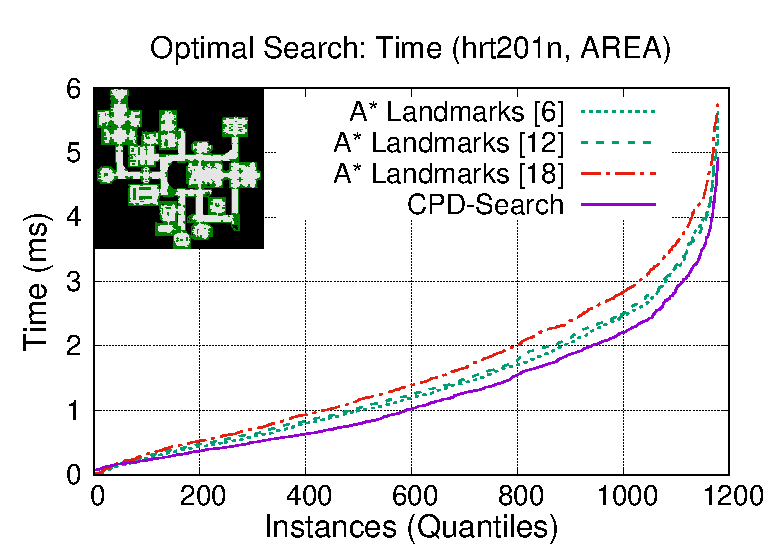
\includegraphics[width=1.0\textwidth]{src/images/pathfinding/optimal/hrt201n}
            \end{figure}
        \end{minipage}
    \end{adjustwidth}
\end{frame}